% Options for packages loaded elsewhere
\PassOptionsToPackage{unicode}{hyperref}
\PassOptionsToPackage{hyphens}{url}
%
\documentclass[
]{article}
\usepackage{lmodern}
\usepackage{amssymb,amsmath}
\usepackage{ifxetex,ifluatex}
\ifnum 0\ifxetex 1\fi\ifluatex 1\fi=0 % if pdftex
  \usepackage[T1]{fontenc}
  \usepackage[utf8]{inputenc}
  \usepackage{textcomp} % provide euro and other symbols
\else % if luatex or xetex
  \usepackage{unicode-math}
  \defaultfontfeatures{Scale=MatchLowercase}
  \defaultfontfeatures[\rmfamily]{Ligatures=TeX,Scale=1}
\fi
% Use upquote if available, for straight quotes in verbatim environments
\IfFileExists{upquote.sty}{\usepackage{upquote}}{}
\IfFileExists{microtype.sty}{% use microtype if available
  \usepackage[]{microtype}
  \UseMicrotypeSet[protrusion]{basicmath} % disable protrusion for tt fonts
}{}
\makeatletter
\@ifundefined{KOMAClassName}{% if non-KOMA class
  \IfFileExists{parskip.sty}{%
    \usepackage{parskip}
  }{% else
    \setlength{\parindent}{0pt}
    \setlength{\parskip}{6pt plus 2pt minus 1pt}}
}{% if KOMA class
  \KOMAoptions{parskip=half}}
\makeatother
\usepackage{xcolor}
\IfFileExists{xurl.sty}{\usepackage{xurl}}{} % add URL line breaks if available
\IfFileExists{bookmark.sty}{\usepackage{bookmark}}{\usepackage{hyperref}}
\hypersetup{
  pdftitle={Test UMLR},
  pdfauthor={Javier Gonzalez},
  hidelinks,
  pdfcreator={LaTeX via pandoc}}
\urlstyle{same} % disable monospaced font for URLs
\usepackage[margin=1in]{geometry}
\usepackage{color}
\usepackage{fancyvrb}
\newcommand{\VerbBar}{|}
\newcommand{\VERB}{\Verb[commandchars=\\\{\}]}
\DefineVerbatimEnvironment{Highlighting}{Verbatim}{commandchars=\\\{\}}
% Add ',fontsize=\small' for more characters per line
\usepackage{framed}
\definecolor{shadecolor}{RGB}{248,248,248}
\newenvironment{Shaded}{\begin{snugshade}}{\end{snugshade}}
\newcommand{\AlertTok}[1]{\textcolor[rgb]{0.94,0.16,0.16}{#1}}
\newcommand{\AnnotationTok}[1]{\textcolor[rgb]{0.56,0.35,0.01}{\textbf{\textit{#1}}}}
\newcommand{\AttributeTok}[1]{\textcolor[rgb]{0.77,0.63,0.00}{#1}}
\newcommand{\BaseNTok}[1]{\textcolor[rgb]{0.00,0.00,0.81}{#1}}
\newcommand{\BuiltInTok}[1]{#1}
\newcommand{\CharTok}[1]{\textcolor[rgb]{0.31,0.60,0.02}{#1}}
\newcommand{\CommentTok}[1]{\textcolor[rgb]{0.56,0.35,0.01}{\textit{#1}}}
\newcommand{\CommentVarTok}[1]{\textcolor[rgb]{0.56,0.35,0.01}{\textbf{\textit{#1}}}}
\newcommand{\ConstantTok}[1]{\textcolor[rgb]{0.00,0.00,0.00}{#1}}
\newcommand{\ControlFlowTok}[1]{\textcolor[rgb]{0.13,0.29,0.53}{\textbf{#1}}}
\newcommand{\DataTypeTok}[1]{\textcolor[rgb]{0.13,0.29,0.53}{#1}}
\newcommand{\DecValTok}[1]{\textcolor[rgb]{0.00,0.00,0.81}{#1}}
\newcommand{\DocumentationTok}[1]{\textcolor[rgb]{0.56,0.35,0.01}{\textbf{\textit{#1}}}}
\newcommand{\ErrorTok}[1]{\textcolor[rgb]{0.64,0.00,0.00}{\textbf{#1}}}
\newcommand{\ExtensionTok}[1]{#1}
\newcommand{\FloatTok}[1]{\textcolor[rgb]{0.00,0.00,0.81}{#1}}
\newcommand{\FunctionTok}[1]{\textcolor[rgb]{0.00,0.00,0.00}{#1}}
\newcommand{\ImportTok}[1]{#1}
\newcommand{\InformationTok}[1]{\textcolor[rgb]{0.56,0.35,0.01}{\textbf{\textit{#1}}}}
\newcommand{\KeywordTok}[1]{\textcolor[rgb]{0.13,0.29,0.53}{\textbf{#1}}}
\newcommand{\NormalTok}[1]{#1}
\newcommand{\OperatorTok}[1]{\textcolor[rgb]{0.81,0.36,0.00}{\textbf{#1}}}
\newcommand{\OtherTok}[1]{\textcolor[rgb]{0.56,0.35,0.01}{#1}}
\newcommand{\PreprocessorTok}[1]{\textcolor[rgb]{0.56,0.35,0.01}{\textit{#1}}}
\newcommand{\RegionMarkerTok}[1]{#1}
\newcommand{\SpecialCharTok}[1]{\textcolor[rgb]{0.00,0.00,0.00}{#1}}
\newcommand{\SpecialStringTok}[1]{\textcolor[rgb]{0.31,0.60,0.02}{#1}}
\newcommand{\StringTok}[1]{\textcolor[rgb]{0.31,0.60,0.02}{#1}}
\newcommand{\VariableTok}[1]{\textcolor[rgb]{0.00,0.00,0.00}{#1}}
\newcommand{\VerbatimStringTok}[1]{\textcolor[rgb]{0.31,0.60,0.02}{#1}}
\newcommand{\WarningTok}[1]{\textcolor[rgb]{0.56,0.35,0.01}{\textbf{\textit{#1}}}}
\usepackage{longtable,booktabs}
% Correct order of tables after \paragraph or \subparagraph
\usepackage{etoolbox}
\makeatletter
\patchcmd\longtable{\par}{\if@noskipsec\mbox{}\fi\par}{}{}
\makeatother
% Allow footnotes in longtable head/foot
\IfFileExists{footnotehyper.sty}{\usepackage{footnotehyper}}{\usepackage{footnote}}
\makesavenoteenv{longtable}
\usepackage{graphicx,grffile}
\makeatletter
\def\maxwidth{\ifdim\Gin@nat@width>\linewidth\linewidth\else\Gin@nat@width\fi}
\def\maxheight{\ifdim\Gin@nat@height>\textheight\textheight\else\Gin@nat@height\fi}
\makeatother
% Scale images if necessary, so that they will not overflow the page
% margins by default, and it is still possible to overwrite the defaults
% using explicit options in \includegraphics[width, height, ...]{}
\setkeys{Gin}{width=\maxwidth,height=\maxheight,keepaspectratio}
% Set default figure placement to htbp
\makeatletter
\def\fps@figure{htbp}
\makeatother
\setlength{\emergencystretch}{3em} % prevent overfull lines
\providecommand{\tightlist}{%
  \setlength{\itemsep}{0pt}\setlength{\parskip}{0pt}}
\setcounter{secnumdepth}{-\maxdimen} % remove section numbering

\title{Test UMLR}
\author{Javier Gonzalez}
\date{22/8/2020}

\begin{document}
\maketitle

\begin{Shaded}
\begin{Highlighting}[]
\KeywordTok{print}\NormalTok{(}\KeywordTok{cat}\NormalTok{(}\StringTok{"Inicio desde "}\NormalTok{, }\KeywordTok{getwd}\NormalTok{()))}
\end{Highlighting}
\end{Shaded}

\begin{verbatim}
## Inicio desde  C:/Data/PRJ/R/umlr2/testsNULL
\end{verbatim}

\begin{Shaded}
\begin{Highlighting}[]
\CommentTok{# umlr$addStyle("monochrome", TRUE)}
\CommentTok{# base = UMLShow$complete + UMLShow$subclasses + UMLShow$parents + UMLShow$classComplete}
\CommentTok{# umlr$plotClass(c10, base)}
\end{Highlighting}
\end{Shaded}

\hypertarget{intro}{%
\section{Intro}\label{intro}}

El paquete provee una clase (\textbf{UMLR}) para generar definiciones
UML de objetos R. Actualmente es posible procesar:

\begin{itemize}
\tightlist
\item
  Clases R6
\item
  Clases S4
\end{itemize}

El proceso general consiste en crear un objeto \textbf{UMLR} y ejecutar
el método uno de los siguientes métodos sobre una instancia de una clase
o un vector de ellas:

\begin{itemize}
\tightlist
\item
  plot
\end{itemize}

\hypertarget{parametros-de-control}{%
\section{Parametros de control}\label{parametros-de-control}}

El nivel de detalle y la información a generar se gestiona a través de
los siguientes parámetros:

\begin{itemize}
\tightlist
\item
  detail
\item
  deep
\end{itemize}

\hypertarget{nivel-de-informaciuxf3n-detail}{%
\subsection{\texorpdfstring{Nivel de información:
\emph{detail}}{Nivel de información: detail}}\label{nivel-de-informaciuxf3n-detail}}

\begin{longtable}[]{@{}lrl@{}}
\toprule
\begin{minipage}[b]{0.15\columnwidth}\raggedright
Nombre\strut
\end{minipage} & \begin{minipage}[b]{0.06\columnwidth}\raggedleft
Valor\strut
\end{minipage} & \begin{minipage}[b]{0.70\columnwidth}\raggedright
Muestra\strut
\end{minipage}\tabularnewline
\midrule
\endhead
\begin{minipage}[t]{0.15\columnwidth}\raggedright
basic\strut
\end{minipage} & \begin{minipage}[t]{0.06\columnwidth}\raggedleft
0\strut
\end{minipage} & \begin{minipage}[t]{0.70\columnwidth}\raggedright
Miembros publicos propios y heredados\strut
\end{minipage}\tabularnewline
\begin{minipage}[t]{0.15\columnwidth}\raggedright
simple\strut
\end{minipage} & \begin{minipage}[t]{0.06\columnwidth}\raggedleft
1\strut
\end{minipage} & \begin{minipage}[t]{0.70\columnwidth}\raggedright
Miembros publicos propios\strut
\end{minipage}\tabularnewline
\begin{minipage}[t]{0.15\columnwidth}\raggedright
complete\strut
\end{minipage} & \begin{minipage}[t]{0.06\columnwidth}\raggedleft
2\strut
\end{minipage} & \begin{minipage}[t]{0.70\columnwidth}\raggedright
Todos los miembros de la clase\strut
\end{minipage}\tabularnewline
\begin{minipage}[t]{0.15\columnwidth}\raggedright
superClasses\strut
\end{minipage} & \begin{minipage}[t]{0.06\columnwidth}\raggedleft
16\strut
\end{minipage} & \begin{minipage}[t]{0.70\columnwidth}\raggedright
La clase de la que hereda (si existe)\strut
\end{minipage}\tabularnewline
\begin{minipage}[t]{0.15\columnwidth}\raggedright
subClasses\strut
\end{minipage} & \begin{minipage}[t]{0.06\columnwidth}\raggedleft
32\strut
\end{minipage} & \begin{minipage}[t]{0.70\columnwidth}\raggedright
Las clases que usa (agregadas o compuestas)\strut
\end{minipage}\tabularnewline
\begin{minipage}[t]{0.15\columnwidth}\raggedright
classSimple\strut
\end{minipage} & \begin{minipage}[t]{0.06\columnwidth}\raggedleft
256\strut
\end{minipage} & \begin{minipage}[t]{0.70\columnwidth}\raggedright
Igual que `simple' pero aplicado a las superclases y subclases\strut
\end{minipage}\tabularnewline
\begin{minipage}[t]{0.15\columnwidth}\raggedright
classComplete\strut
\end{minipage} & \begin{minipage}[t]{0.06\columnwidth}\raggedleft
512\strut
\end{minipage} & \begin{minipage}[t]{0.70\columnwidth}\raggedright
Igual que `complete' pero aplicado a las superclases y subclases\strut
\end{minipage}\tabularnewline
\bottomrule
\end{longtable}

\hypertarget{profundidad-de-analisis-deep}{%
\subsection{\texorpdfstring{Profundidad de analisis:
\emph{deep}}{Profundidad de analisis: deep}}\label{profundidad-de-analisis-deep}}

Cuando tiene sentido; es decir, cuando se ha indicado que se muestren
super o subclases, \emph{deep} indica en nivel de profundidad del
análisis.

Ejemplo:

Supongamos la siguiente estructura de clases:

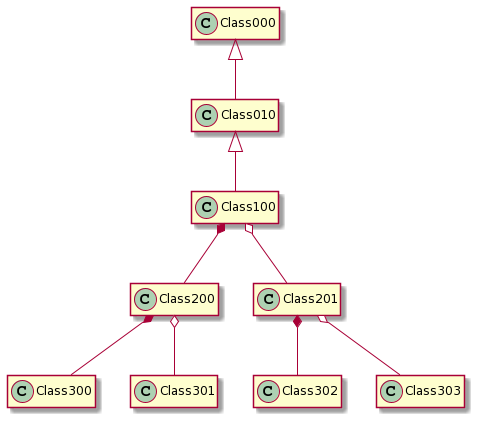
\includegraphics[width=6.69in]{../vignettes/img/jerarquia}

\begin{verbatim}
## Called from: container$getDefinition()
## debug: uml = generateHeaders()
## debug: for (pkg in getPackages()) uml = c(uml, pkg$definition())
## debug: classes = getClasses()
## debug: if (length(classes) > 0) {
##     for (cls in classes) uml = c(uml, cls$definition())
##     parents = lapply(seq(1, length(classes)), function(x) classes[[x]]$getParentsRelation())
##     uml = c(uml, unique(unlist(parents)))
##     sons = lapply(seq(1, length(classes)), function(x) classes[[x]]$getSubclassesRelation())
##     uml = c(uml, unique(unlist(sons)))
## }
## debug: relations = NULL
## debug: rels = getRelations()
## debug: if (length(rels) > 0) relations = lapply(rels, function(x) x$definition())
## debug: relations = lapply(rels, function(x) x$definition())
## debug: c(uml, relations)
\end{verbatim}

\includegraphics[width=8.26in]{C:\tmp\Rtmp4OtfIh\file310c37b63240}

umlr\(plotClass(c(uml, umlr), UMLShow\)basic)

simple

umlr\(plotClass(c(uml, umlr), UMLShow\)simple)

con padres

base = UMLShow\(complete + UMLShow\)superClasses umlr\$plotClass(c(uml,
umlr), base)

\hypertarget{paruxe1metro-deep}{%
\subsubsection{\texorpdfstring{parámetro
\emph{deep}}{parámetro deep}}\label{paruxe1metro-deep}}

completo

base = UMLShow\(complete + UMLShow\)superClasses +
UMLShow\(subClasses umlr\)plotClass(c(uml, umlr), base +
UMLShow\$classComplete, deep=10)

UMLShow\$

Supongamos la siguiente clase sencilla

\begin{Shaded}
\begin{Highlighting}[]
\NormalTok{Class00 =}\StringTok{ }\NormalTok{R6}\OperatorTok{::}\KeywordTok{R6Class}\NormalTok{(}\StringTok{"R6CLASS00"}\NormalTok{,}
 \DataTypeTok{public =} \KeywordTok{list}\NormalTok{(}
    \DataTypeTok{initialize =} \ControlFlowTok{function}\NormalTok{(...) \{ \}}
\NormalTok{   ,}\DataTypeTok{method00   =} \ControlFlowTok{function}\NormalTok{()    \{ \}}
\NormalTok{ )}
\NormalTok{ ,}\DataTypeTok{active  =} \KeywordTok{list}\NormalTok{ (}
     \DataTypeTok{var00 =} \ControlFlowTok{function}\NormalTok{(value) \{ \}}
\NormalTok{ )}
\NormalTok{ ,}\DataTypeTok{private =} \KeywordTok{list}\NormalTok{ (}
      \DataTypeTok{.var00    =} \OtherTok{NA}
\NormalTok{     ,}\DataTypeTok{.method00 =} \ControlFlowTok{function}\NormalTok{(data) \{\}}
\NormalTok{ )}
\NormalTok{)}
\NormalTok{c00 =}\StringTok{ }\NormalTok{Class00}\OperatorTok{$}\KeywordTok{new}\NormalTok{()}
\end{Highlighting}
\end{Shaded}

umlrr = UMLR\$new(plantuml = ``c:/SDK/plantuml/plantuml.jar'' ,inputDir
= ``uml'' ,outputDir = ``img'' )

umlrr\(addClass(c00)  umlrr\)plot()

\#rc = uml\$checkInstallation()

\hypertarget{monochrome}{%
\subsection{monochrome}\label{monochrome}}

print(``Antes'')

\hypertarget{umlraddstylemonochrome-true}{%
\section{umlr\$addStyle(``monochrome'',
TRUE)}\label{umlraddstylemonochrome-true}}

\end{document}
